\documentclass[a4paper]{report}

\usepackage[utf8]{inputenc}
\usepackage[portuges]{babel}
\usepackage{a4wide}
\usepackage{graphicx}
\usepackage{amsmath}
\usepackage{mathtools}

\title{Projeto de Laboratórios de Informática I\\Grupo 168}
\author{Alexandre Mendonça Pinho (82441) \and Joel Filipe Esteves Gama (82202)}
\date{\today}

\begin{document}
\maketitle
\begin{abstract}
Neste relatório é apresentada uma introdução ao projeto. Nele é, também, descrito o problema a resolver, explicamos a nossa conceção da solução, esta dividida em três secções, \emph{Estruturas de Dados}, \emph{Implementeção} e \emph{Testes} e por fim uma conclusão do relatório, onde é feita uma análise crítica com base nos resultados obtidos.

Desta forma apresentamos a nossa solução para o problema em questão (desenvolvimento do jogo Bomberman em linguagem de programação funcional \textit{Haskell}), os resultados obtidos bem como as conclusões retiradas a partir dos mesmos.
\end{abstract}
\tableofcontents
\chapter{Introdução}
\label{sec:intro}
Este relatório apresenta uma descrição e explicação do projeto da disciplina de Laboratórios de Informática I (LI I),
do 1º ano do Mestrado Integrado em Engenharia Informática da Universidade do Minho (MIEI - UM),
que toma a forma de um projeto a ser desenvolvido na linguagem de programação funcional \textit{Haskell}.

Com o objectivo de fazer um clone do jogo Bomberman e um \textit{bot} para jogar o jogo, as primeiras tarefas constituem as bases do jogo, e só depois foi implementada a parte gráfica. Para a parte gráfica utilizamos a \textit{framework} do \textit{Gloss} com auxílio da biblioteca \textit{gloss-juicy} para poder utilizar o formato de imagem PNG.

Na tarefa 6, a filosofia AI do grupo fez com que o comportamento do \textit{bot} não fosse \textit{'hardcoded'} mas sim emergente de várias componentes do "pensamento" do \textit{bot}, permitindo também uma fácil alteração do mesmo.

O relatório apresenta um breve resumo do mesmo, como um preâmbulo, introdução, seguida de uma descrição do problema, apresentação da proposta de resolução e por fim a conclusão, onde é feita uma análise crítica dos resultados.
\chapter{Descrição do Problema}
\label{sec:problema}
O problema levantado (desenvolvimento do jogo Bomberman em linguagem de programação funcional \textit{Haskell}) implica que tenhamos de escrever várias tarefas de código, para que o jogo funcione. Desta forma o jogo é maioritariamente escrita de código e também uma parte de desenho (\textit{Pixel Art}). Assim sendo, foi necessário aplicar os conhecimentos adquiridos nas aulas de Programação Funcional e também alguns adquiridos por pesquisa autónoma para que conseguíssemos por o jogo a funcionar.

O projeto está dividido em seis tarefas, e estas distribuídas em duas fases, tarefas 1, 2 e 3 correspondentes à primeira fase e tarefas 4, 5 e 6 correspondentes à segunda fase. As três primeiras tarefas foram utilizadas para a geração de mapas, definição de comandos e compressão de código (tarefas 1, 2 e 3, respetivamente). Já estas últimas tarefas são para passagem do tempo, criação de gráficos para o funcionamento do jogo e criação de um \textit{bot} (tarefas 4, 5 e 6, respetivamente).

Em cada umas das tarefas é pretendido um objetivo diferente. Na primeira fase: a tarefa 1 tem como objetivo a criação de mapas, ou seja, atribuindo uma dimensão e uma semente o mapa era gerado com um número e localizações aleatórias de \textit{PowerUps}, a tarefa 2 pretende a reação a comandos, isto é, fazer com que o jogador se mova e coloque bombas, e para finalizar a primeira fase temos a tarefa 3 utilizada para fazer a compressão do código. Já na segunda fase do projeto: na tarefa 4 a passagem de tempo, é pretendido que se desenvolva funções que façam com que o tempo avance, o que, por consequência faz que as bombas explodam, e no caso de os jogadores estarem sob a influência de um comando faz com que os mesmos se movam, a tarefa 5 tem como objetivo a criação da interface gráfica para o jogo, ou seja, o desenvolvimento de funções utilizando o \textit{Gloss} (o \textit{Gloss} é uma biblioteca \textit{Haskell} minimalista para a criação de gráficos e animações 2D) para que as imagens, criadas à parte utilizando um editor de imagens (\textit{GIMP}, no nosso caso), possam ser utilizadas no mapa, e por fim, a tarefa 6, criação de um \textit{bot}, pretende que sejam criados comandos (funções) para que o jogador possa funcionar de forma autónoma e não precise de estar a ser controlado por uma pessoa, uma vez que os comandos são executados automaticamente segundo uma lista de prioridade.
\chapter{Conceção da Solução}
\label{sec:solucao}
\section{Estruturas de Dados}
Nas tarefas 1, 2 e 3 a estrutura de dados utilizada para representar o mapa do jogo foi a original, uma lista de \textit{Strings}. Tal como nas tarefas 4 e 6.


Já na tarefa 5, o \textit{Estado} (nome atribuído ao estado do jogo) incluía uma lista de listas de \textit{Tiles}, para representar os blocos do mapa, uma lista de \textit{Powerups}, uma lista de bombas, uma lista de jogadores, uma lista de \textit{Blasts} e também os instantes restantes até ao final da partida (estes representados por um \textit{Float}).

Nas listas criadas existe uma identificação específica dos tipos do seu conteúdo. Na lista de listas de \textit{Tiles} existem os seguistes tipos: \textit{Rock} que representam as rochas existentes (tanto exteriores, como interiores), \textit{Empty} que representa os blocos que não contêm nada, \textit{Brick} que representa os tijolos que podem ser removidos e podem, também, esconder \textit{Powerups} e existem \textit{RemovedTile} que representam os \textit{Tiles} que foram removidos do mapa, como por exemplo, tijolos. 

Na lista dos \textit{Powerups} estão definidos três tipos de \textit{Powerups}: \textit{BombPW} a representar os \textit{Powerups} bomba, \textit{FlamePW} a representar os \textit{PowerUps} flame e \textit{RemovedPW} que representa os \textit{Powerups} removidos. A lista de \textit{PowerUps}0 é constituída por tuplos, em que o primeiro elemento é o tipo de \textit{Powerup} e o segundo é um par de coordenadas que informa qual posição do \textit{Powerup} \textbf{(PWType,Pos)}.

Na descrição do estado segue-se uma lista de bombas que é composta por todas as bombas que se encontram no mapa naquele preciso instante do jogo. Uma \textit{Bomb} é o correspondente a uma bomba e é constituída pela sua posição, o número do jogador que a colocou, o raio de explosão e o instantes de tempo até à explosão \textbf{(Pos,Int,Int,Int)}.

Na lista de jogadores, cada jogador está definido com o seu número, a sua posição, um tuplo que representa o numero de \textit{Powerups} bomb e flames, respetivamente, um tipo chamado de \textit{Motion} que representa os comandos possíveis aos jogadores efetuarem e um \textit{Either}, que decide se o jogador é controlado por uma pessoa, ou por um \textit{bot} \textbf{(Int,Pos,(Int,Int),Motion,(Either (Key,Key,Key,Key,Key) ([String] -\textgreater Int -\textgreater Int -\textgreater Maybe -\textgreater Char))))}.

A penúltima componente do estado do jogo é uma lista de \textit{Blasts} que representa as explosões das bombas, esta lista é utilizada para a impressão no mapa da explosão das bombas.

Assim, a estrutura de dados utilizada no nosso projeto resume-se ao que foi descrito anteriormente.
\section{Implementação}
\subsection{Tarefa 1}
A implementação da tarefa 1 é separada em três passos: a geração dos carateres do mapa, a geração das linhas dos \textit{Powerups} bomba, e a geração das linhas dos \textit{Powerups} flame. No primeiro passo, é gerado o mapa através de chamadas recursivas para as linhas, que por sua vez são geradas através de chamadas recursivas, determinando os conteúdos dos blocos um por um. Os blocos predefinidos são determinados ao testar cada posição: se for uma posição na borda do mapa ou em posições de linhas e colunas pares (contando a partir do zero) é pedra, e se pertencer a uma lista de espaços vazios definida globalmente é vazio.

Os dois últimos passos são separados devido à necessidade de introduzir as linhas dos dois tipos de \textit{Powerup} separadamente. No entanto, como a especificação da tarefa indica que o método de determinação do conteúdo de um bloco, tanto em termos de estar vazio, ou com um tijolo ou uma pedra, como em termos de ter ou não um \textit{Powerup}, foi necessário 'marcar' no output do primeiro passo, para além das pedras (representadas por cardinais), dos tijolos (pontos de interrogação) e dos espaços vazios (espaços), as posições onde se encontra um \textit{Powerup} e o seu respetivo tipo, introduzindo um sinal mais no caso de ser \textit{Powerup} bomba, e um ponto de exclamação no caso de ser \textit{Powerup} flame. Este output é passado como argumento para as funções que geram as linhas dos \textit{Powerups}, e no fim é incluído no output da função mapa, mas sem as tais marcas, substituindo-as por pontos de interrogação.

\subsection{Tarefa 2}
Na tarefa 2, cada comando é tratado por um função diferente. Para os comandos de movimento do jogador ('U','D','L', e 'R'), o procedimento é similar: o jogador apenas é movido se a posição para onde ele se pretende mover estiver vazia, isto é, se não existir uma pedra ou um tijolo. Se este for o caso, é retornado um novo conjunto de \textit{Strings} onde muda a posição do jogador, e caso exista um \textit{Powerup} na nova posição, ele é retirado do mapa e adicionado ao jogador (acrescentando um sinal mais ou um ponto de exclamação após o terceiro espaço da linha do jogador ou no fim da mesma, respetivamente).

\subsection{Tarefa 3}
Na tarefa 3, a principal estratégia de compressão, depois da removimento dos blocos fixos, foi a utilização de um único bit (onde cada 8 bits formam um carater no \textit{String} final) para representar espaços vazios (0) ou tijolos (1) no conjunto de posições não pré-definidas. O formato comprimido (por ordem) é o seguinte (com o número de bits ocupado por cada parte à frente):

\begin{itemize}
\item Dimensão - 7 \textit{bits}
\item \textit{Bits} dos blocos não pré-definidos - número de blocos não pré-definidos \footnote{d \^\ 2 - 4 \* (d - 1) - 12 - (div (d - 3) 2) \^\ 2

\textbf{formula para o cálculo do número de blocos não pré-definidos, onde d é a dimensão do mapa.}}
\item Número de \textit{Powerups} - 9 \textit{bits}
\item \textit{Powerups} - 15 \textit{bits} por cada (1 \textit{bit} para o tipo, e 7 \textit{bits} para cada coordenada)
\item Número de bombas - 7 \textit{bits}
\item Bombas - 27 \textit{bits} por cada (7 \textit{bits} para cada coordenada, 2 \textit{bits} para o número do jogador, 7 \textit{bits} para o tamanho da explosão, e 4 \textit{bits} para os instantes de tempo que faltam até a bomba explodir)
\item Tabela de jogadores - 8 \textit{bits} (2 \textit{bits} para cada um dos 4 jogadores, o primeiro \textit{bit} indica a existência do jogador e o segundo se ele tem \textit{Powerups} acumulados)
\item Jogadores - 14 \textit{bits} por cada jogador sem \textit{Powerups} (7 \textit{bits} para cada coordenada), e 28 \textit{bits} por cada jogador com \textit{Powerups} (mais 7 \textit{bits} para a contagem de cada tipo de \textit{Powerup}).
\end{itemize}

Após construir este conjunto de \textit{bits}, cada 8 \textit{bits} são transformados em 1 carater (na codificação \textit{ASCII}). Se restarem \textit{bits}, são adicionados 0s até perfazerem 8 (o que não influenciará de qualquer modo o processo de descodificação).

Na descodificação, é primeiramente contruído um mapa de maneira semelhante à da tarefa um (bloco por bloco), mas neste caso não é necessário determinar os conteúdos de um bloco todos de uma vez. Então, são apenas passados como argumento os bits dos blocos não pré-definidos à função que faz os blocos do mapa. De seguida são contruídos os \textit{Powerups}, que por estarem em ordem no mapa inicial ficam em ordem ao descodificar em esforço adicional, as bombas, e por fim os jogadores. Neste último passo, são filtradas as linhas vazias que a função gera quando um certo jogador não existe.

\subsection{Tarefa 4}
Na quarta tarefa, o primeiro passo na implementação do avançar do tempo é a introdução de pedras em forma de espiral caso faltem menos de um certo número de ticks que varia com a dimensão do mapa assim que no fim do jogo, apenas o bloco central não terá sido afetado por este processo. De seguida, separam-se as bombas que explodem no presente instante de tempo das que não explodem, decrescendo o contador por um a estas últimas.

Depois, para cada bomba, é chamada uma função que produz um mapa onde se sentem os efeitos da explosão da bomba, partindo da sua posição central para fora nas quatro direções cartesianas até chegar ao limite da explosão (o raio da explosão), ou até encontrar um tijolo, um \textit{Powerup} ou uma pedra. No caso de encontrar um tijolo ou um \textit{Powerup}, o mapa produzido vem marcado com um 'X' na posição do tijolo (substituindo o ponto de interrogação) ou na linha do \textit{Powerup} (substituindo o carater inicial), para prevenir que um bomba processado posteriormente passe por essas posições e no caso do tijolo, também para prevenir a explosão de um \textit{Powerup} caso ele se encontra na mesma posição.

Finalmente, são removidas todas as marcas do mapa na parte dos blocos (substituindo por um espaço) e dos \textit{Powerups} (removendo a linha por inteiro).

\subsection{Tarefa 5}
Na tarefa 5, ao utilizar as estruturas de dados que descritas anteriormente neste relatório, é necessária para a utilização do código escrito na tarefa 1, a) a separação do mesmo para um ficheiro à parte, b) a definição de uma função que converte o formato do mapa na tarefa 1 para o formato dele na tarefa 5, e c) a definição de uma semente aleatória (concretizado através da função \textit{randomRIO}).

Com o mapa definido, são adicionados os vários jogadores, que podem ser humanos com controlados pelo \textit{bot} feito na tarefa 6 (ou por qualquer outro, com ligeiras alterações no código). Esta \textit{feature} do jogo é conseguida através do datatype \textit{Either}, processando de diferentes maneiras os tipos (se o construtor for Left, são aceites 5 teclas para um humano controlar o jogador, movendo-o o pondo bombas; caso o construtor seja Right, é aceite uma função com o tipo pedido na tarefa 6 para o \textit{bot}).

A função que desenha o estado do jogo ou desenha um simples menu inicial, ou desenha o mapa do jogo já quando este teve início. Para desenhar os elementos do mapa, primeiro são desenhados os blocos, depois os \textit{Powerups}, seguindo-se as bombas, os jogadores, e por fim as explosões. O grupo achou necessário utilizar o biblioteca \textit{gloss-juicy}, que integra algumas \textit{features} da \textit{framework} \textit{Juicy} no \textit{gloss}, sendo possível utilizar ficheiros de imagem de outros formatos diferentes do formato ".bmp", com o objetivo de ter imagens com transparência no jogo.

Para fazer a atualização do estado do jogo o grupo escolheu não utilizar o código feito nas tarefas 2 e 4, primeiro por ser preciso converter de volta para o formato dessas tarefas, o que despenderia de mais esforço do que a alternativa, e segundo porque existe mais informação dentro do estado do jogo na tarefa 5, especificamente informação necessária para desenhar o estado, que requer menos trabalho incluir no processo de atualização do estado do que determinar no momento da renderização.

\subsection{Tarefa 6}
Na tarefa 6, a estratégia do \textit{bot} é determinada a partir de valores de utilidade das posições para onde é possível o jogador se mover. Para calcular estas, é utilizado um algoritmo "flood fill", considerando da mesma cor os espaços vazios. De seguida, são calculados dois conjuntos de valores de utilidade, uns para o movimento, e outros para as bombas (os dois partindo de um conjunto de valores de utilidade em comum). Devido ao limite de tempo imposto nos testes automáticos dos servidores (e à performance do jogo), os valores de utilidade do movimento são iguais aos valores em comum.

A partir destes valores é determinada a posição para onde o jogador se deve mover e/ou colocar bomba, procurando pelo maior valor em ambos os conjuntos de valores de utilidade. Se esteve valor estiver no conjunto do movimento e jogador se encontra na respetiva posição, o comando será \textit{Nothing}. Se o jogador estiver na posição e for para por uma bomba, o comando é \textit{Just} 'B'. Nos casos onde o jogador não está na posição do valor de utilidade mais alto, é determinado o caminho mais curto para essa posição usando um simples algoritmo que "procura" a posição final nas quatro direções cartesianas (não incluindo caminhos que estão bloqueados, ou que passam por uma posição mais do que uma vez).

Em específico, para calcular os valores de utilidade, são utilizadas três heurísticas: a distância horizontal ou vertical (no caso da posição estar alinhada) de uma (ou várias) bombas, número de tijolos explodidos por uma bomba posta na posição), e a distância ao centro da posição. Dos três, o primeiro e o último são comuns aos dois conjuntos de valores, enquanto o segundo só se aplica aos valores de utilidade para por bombas.

\section{Testes}
Neste projeto criamos vários testes deferentes para testarmos doas as possibilidades de erro nas tarefas. Vamos apenas destacar os três exemplos mais importantes, uma vez que, os restantes são exemplos para correção de erros e verificações básicas.

Começamos pelo Teste 6, este teste foi criado para que fosse possível testar se a espiral estava a funcionar em perfeitas condições, ou seja, testar se a espiral estava a cobrir todos os espaços vazios e também ocupados (com tijolos, bombas e jogadores).

Já a criação do Teste 7 foi para testar se as explosões param em tijolos e em \textit{Powerups}, sendo por essa razão que existe um jogador por trás de um tijolo, pois caso a explosão não pare no tijolo o jogador é morto.

Por fim, o Teste 8 foi criado para testar explosões cruzadas e explosões de bombas em cadeia. 

Estes são os testes mais importantes que foram criados, uma vez que os outros testes apenas testam o passar do tempo e a movimentação dos jogadores (no caso de o jogador a poder fazer) ou a sua imobilidade (no caso de o jogador não se poder mover).
Exemplo disso é o Teste 4.
\begin{figure}[hb]
\begin{center}
    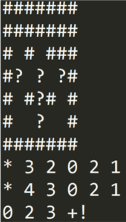
\includegraphics[height=4cm]{Teste6.png} \quad
    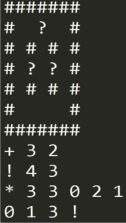
\includegraphics[height=4cm]{Teste7.png} \quad
	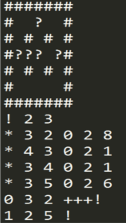
\includegraphics[height=4cm]{Teste8.png} \quad
	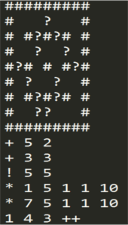
\includegraphics[height=4cm]{Teste4.png}
\caption{Testes 6, 7, 8 e 4, respetivamente} \label{gdimotes}
\end{center}
\end{figure}
\chapter{Conclusão}
\label{sec:conclusao}
Em suma, depois de descrevermos o problema, explica-lo e apresentarmos a nossa proposta de resolução, concluímos que o problema foi resolvido, uma vez que todas as tarefas foram concluídas com sucesso e o jogo funciona, apesar de termos tido algumas dificuldades durante a sua realização. Os resultados obtidos poderiam ter sido melhorados tanto a nível de código, como a nível da interface gráfica do jogo. Isto é, a nível do código, poderíamos ter utilizado algumas funções mais simples, ou até diminuído o número de caracteres utilizados no código, para que, desta forma, o código fosse de melhor leitura e interpretação. Mas para ajudar na tarefa de interpretação (por parte de alguém exterior ao grupo) fizemos a documentação das funções de compreensão mais difícil, ou seja, escrevemos comentários no código que ajudam à interpretação do mesmo. Já a nível da interface gráfica, poderíamos ter melhorado os gráficos desenvolvidos, para que o jogo fica-se com um melhor aspeto, mas não foi possível pela falta de tempo, pois o melhoramento da interface gráfica implicava mais alguns dias de trabalho. Assim, a razão por de trás destas situações que poderiam ter sido melhoradas é a falta de tempo. Mas, apesar disto, o objetivo foi concluído, como já foi referido anteriormente.
\end{document}
